Para problemas como o de otimização de funções, onde o dominio do problema é real, a
representação do cromossomo também pode ser real. Nesse caso, a representação irá
trabalhar diretamente no espaço de busca, sem a necessidade de codificar e decodificar
como no caso binário.

Portanto para representar o problema da otimização da função $f6$, a seguinte configuração foi utilizada:
\begin{itemize}
	\item Representação: Representação real dentro do intervalo $[-100,100]$. Assim, o cromossomo é composto por um vetor de duas posições.

	\item Seleção: Foi utilizados a roleta proporcional ao fitness tanto para a função $f6$
		quanto para a função $f6_{elevada}$.

    \item Operadores genéticos: Para realizar o cruzamento, foi utilizado o algoritmo
    aritmético com uma taxa de cruzamento de 75\%. Também, foi utilizada mutação uniforme
    com uma taxa igual a 1\%.
	\item Critério de paragem: O critério de paragem foi 100 gerações.
\end{itemize}

Assim, foram obtidos os resultados apresentados na tabela \ref{tab:f6_real}.

\begin{table}[htb]
	\centering
	\begin{tabular}{|c|c|c|}
		\hline
		\rowcolor[HTML]{9B9B9B}
		Teste & Média melhor indíviduo & Média população \\\hline
		1 & 0.94825 & 0.89753 \\\hline
		2 & 0.96592 & 0.91702 \\\hline
		3 & 0.95119 & 0.89079 \\\hline
		4 & 0.95656 & 0.90589 \\\hline
		5 & 0.95067 & 0.89339 \\\hline
		\textbf{Média Final} & \textbf{0.954518} & \textbf{0.90092} \\\hline	\end{tabular}
	\caption{Resultados da função $f6$ utilizando representação real, cruzamento aritmético e mutação uniforme \label{tab:f6_real}}
\end{table}

Adicionando elitismo no AG acima, temos um aumento de performance significativo, como mostrado
na tabela~\ref{tab:f6_real_elite}

\begin{table}[htb]
	\centering
	\begin{tabular}{|c|c|c|}
		\hline
		\rowcolor[HTML]{9B9B9B}
		Teste & Média melhor indíviduo & Média população \\\hline
		1 & 0.98896 & 0.94950 \\\hline
		2 & 0.98978 & 0.93423 \\\hline
		3 & 0.98952 & 0.94188 \\\hline
		4 & 0.98867 & 0.94448 \\\hline
		5 & 0.98964 & 0.92809 \\\hline
		\textbf{Média Final} & \textbf{0.98932} & \textbf{0.93963} \\\hline	\end{tabular}
    \caption{Resultados da função $f6$ utilizando representação real, cruzamento aritmético,
    mutação uniforme e elitismo. \label{tab:f6_real_elite}}
\end{table}

\begin{figure}[htb]
	\begin{subfigure}{.45\textwidth}
		\centering
		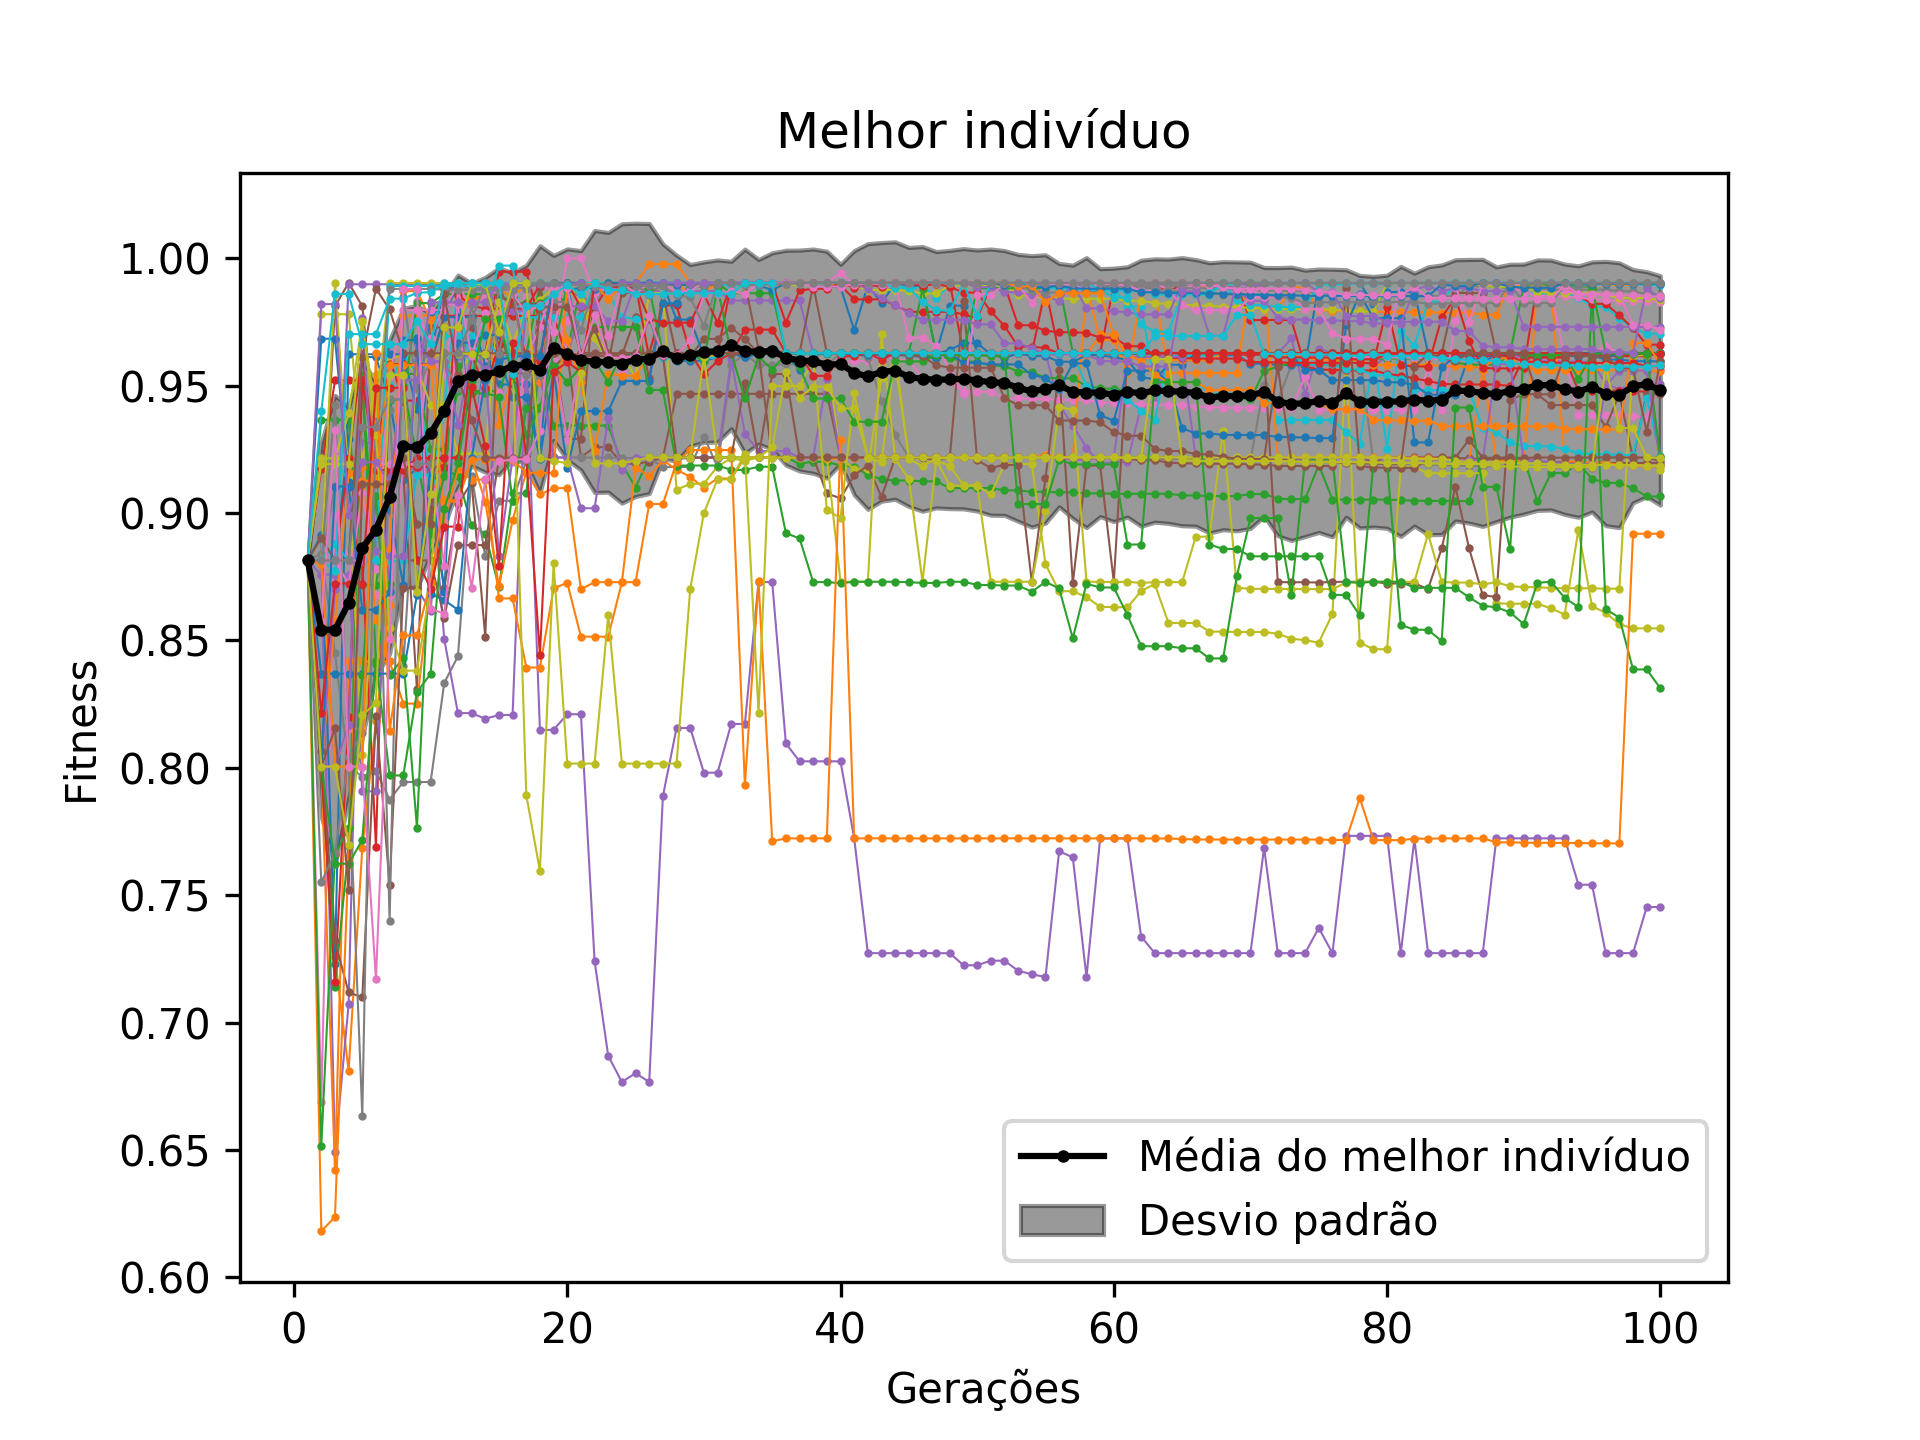
\includegraphics[width=1\textwidth]{sec-03/f6_real_fitness_vs_gen_best.png}
		\caption{Melhores indíviduos de todos os experimentos ao longo das gerações.
		Em preto é mostrado o comportamento médio dos 50 experimentos. }
	\end{subfigure}
	\hfill
	\begin{subfigure}{.45\textwidth}
		\centering
		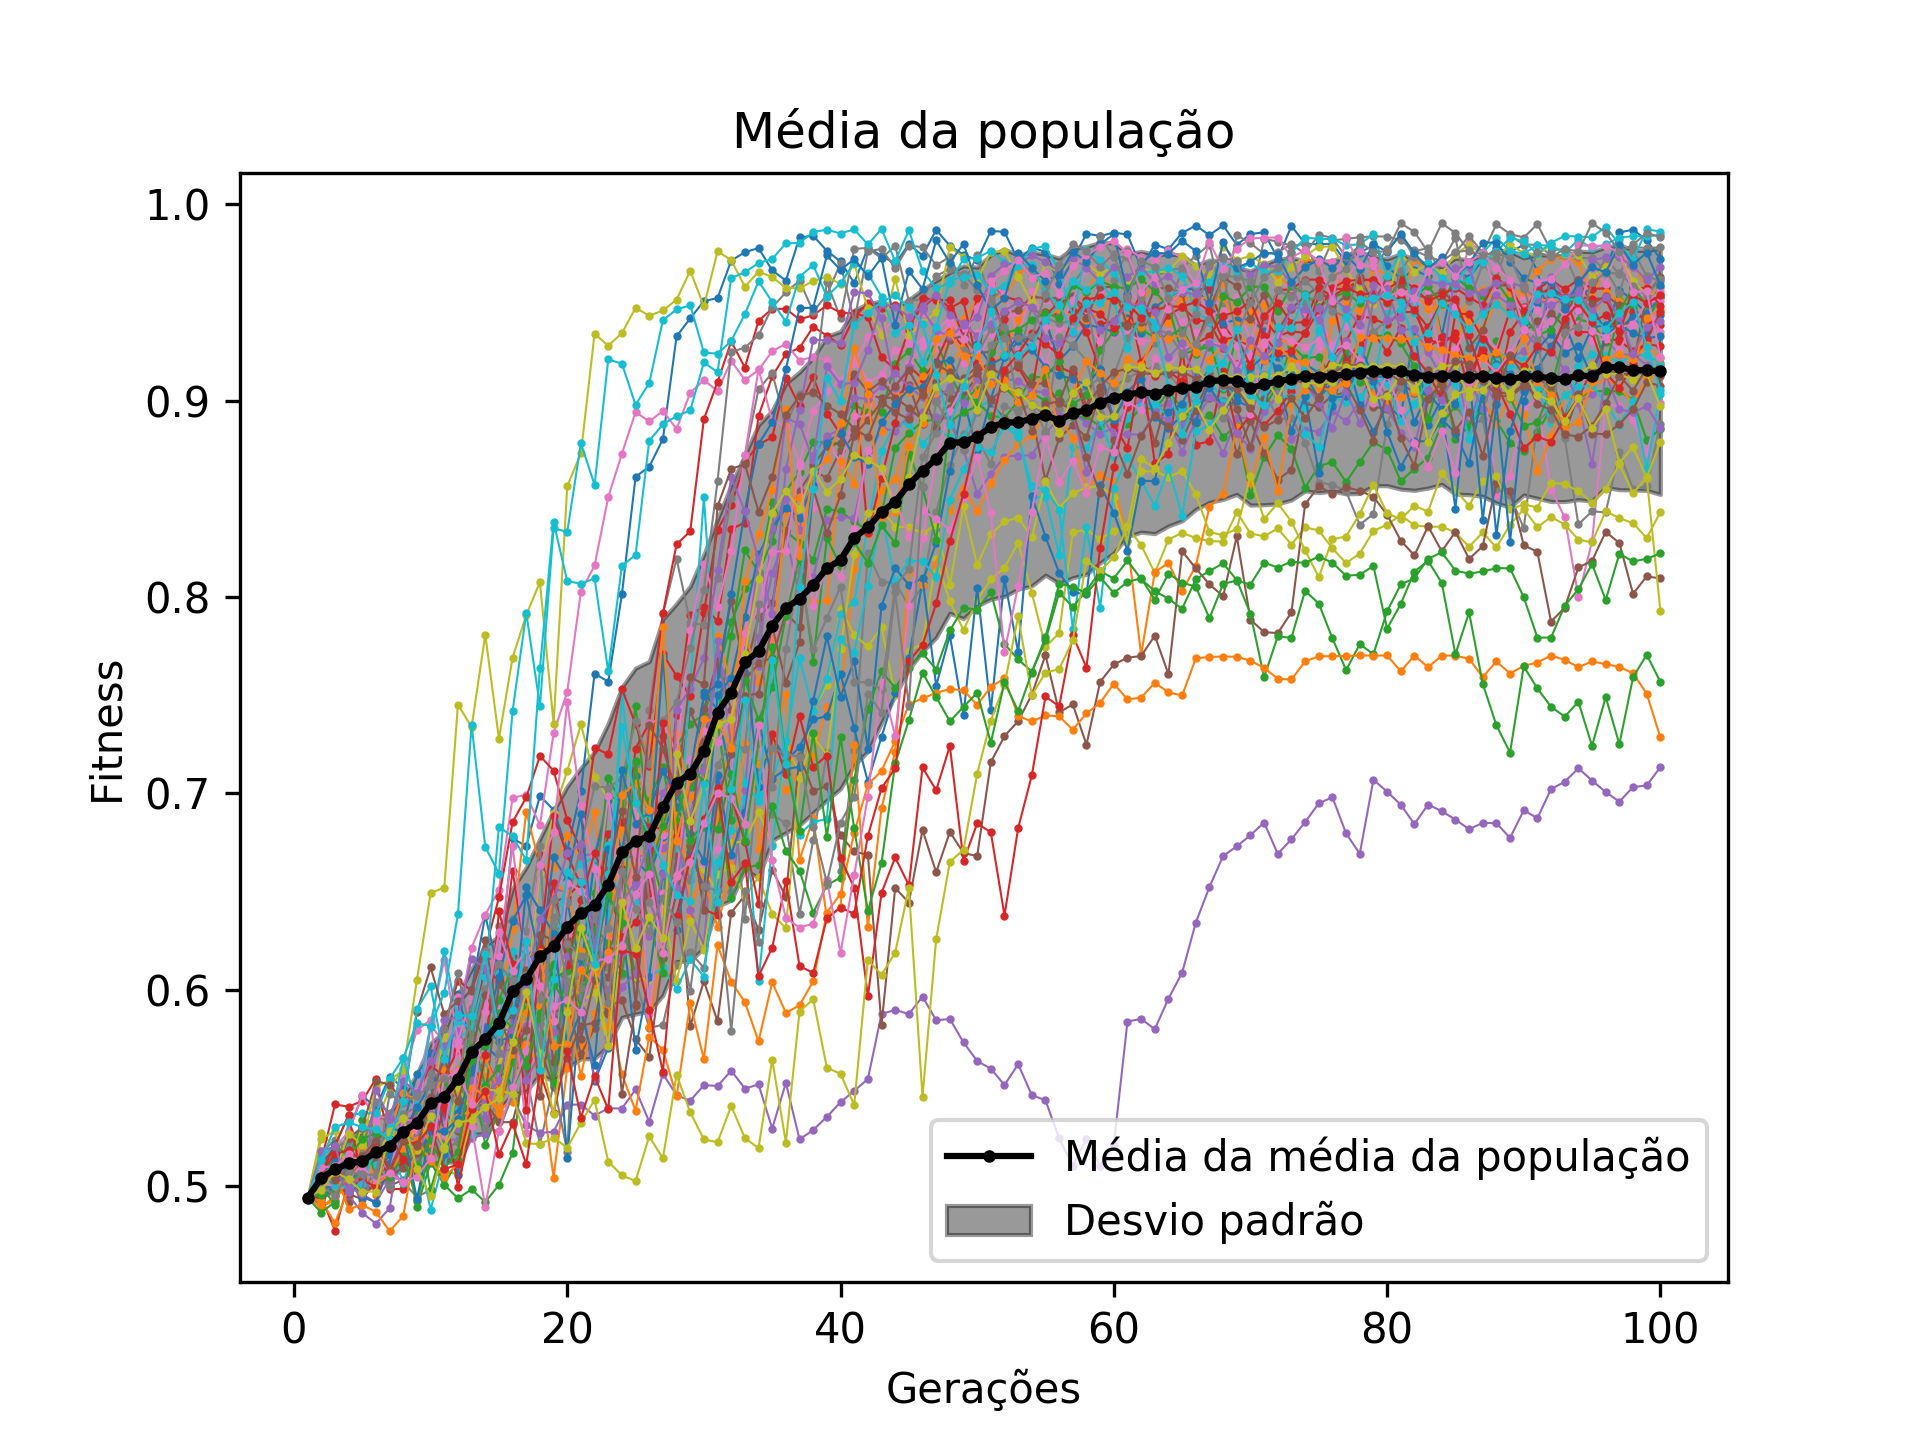
\includegraphics[width=1\textwidth]{sec-03/f6_real_fitness_vs_gen_pop.png}
		\caption{Média da população de todos os experimentos ao longo das gerações.
		Em preto é mostrado o comportamento médio dos 50 experimentos.}
	\end{subfigure}
	\caption{Resultados obtidos utilizando utilizando representação real, cruzamento aritmético e
    mutação uniforme}
\end{figure}


	\begin{figure}[htb]
	\begin{subfigure}{.45\textwidth}
		\centering
		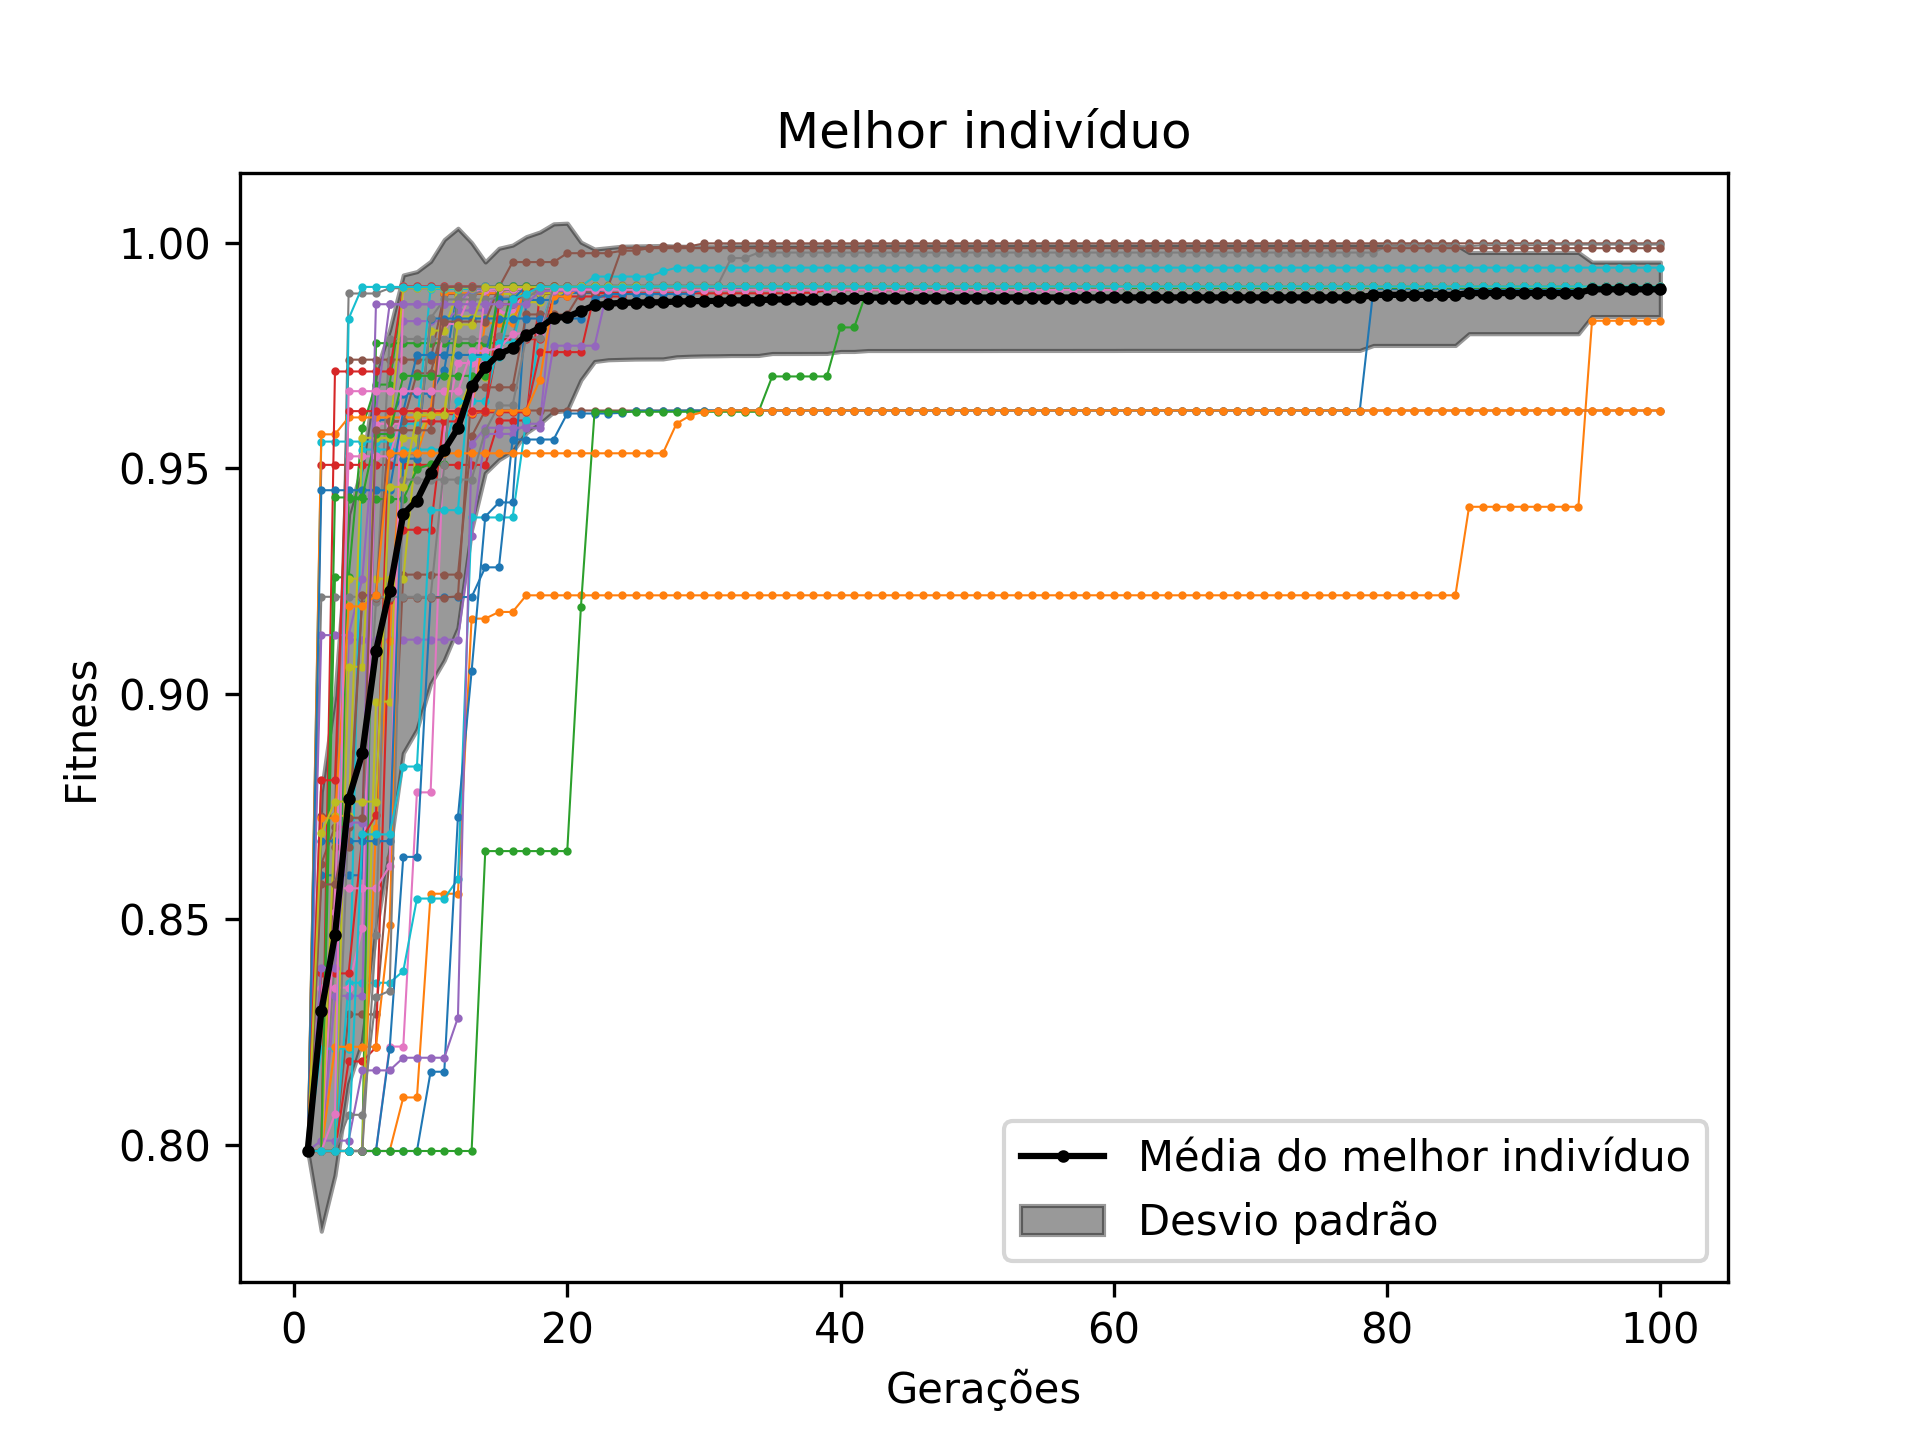
\includegraphics[width=1\textwidth]{sec-03/f6_real_elite_fitness_vs_gen_best.png}
		\caption{Melhores indíviduos de todos os experimentos ao longo das gerações.
		Em preto é mostrado o comportamento médio dos 50 experimentos. }
	\end{subfigure}
	\hfill
	\begin{subfigure}{.45\textwidth}
		\centering
		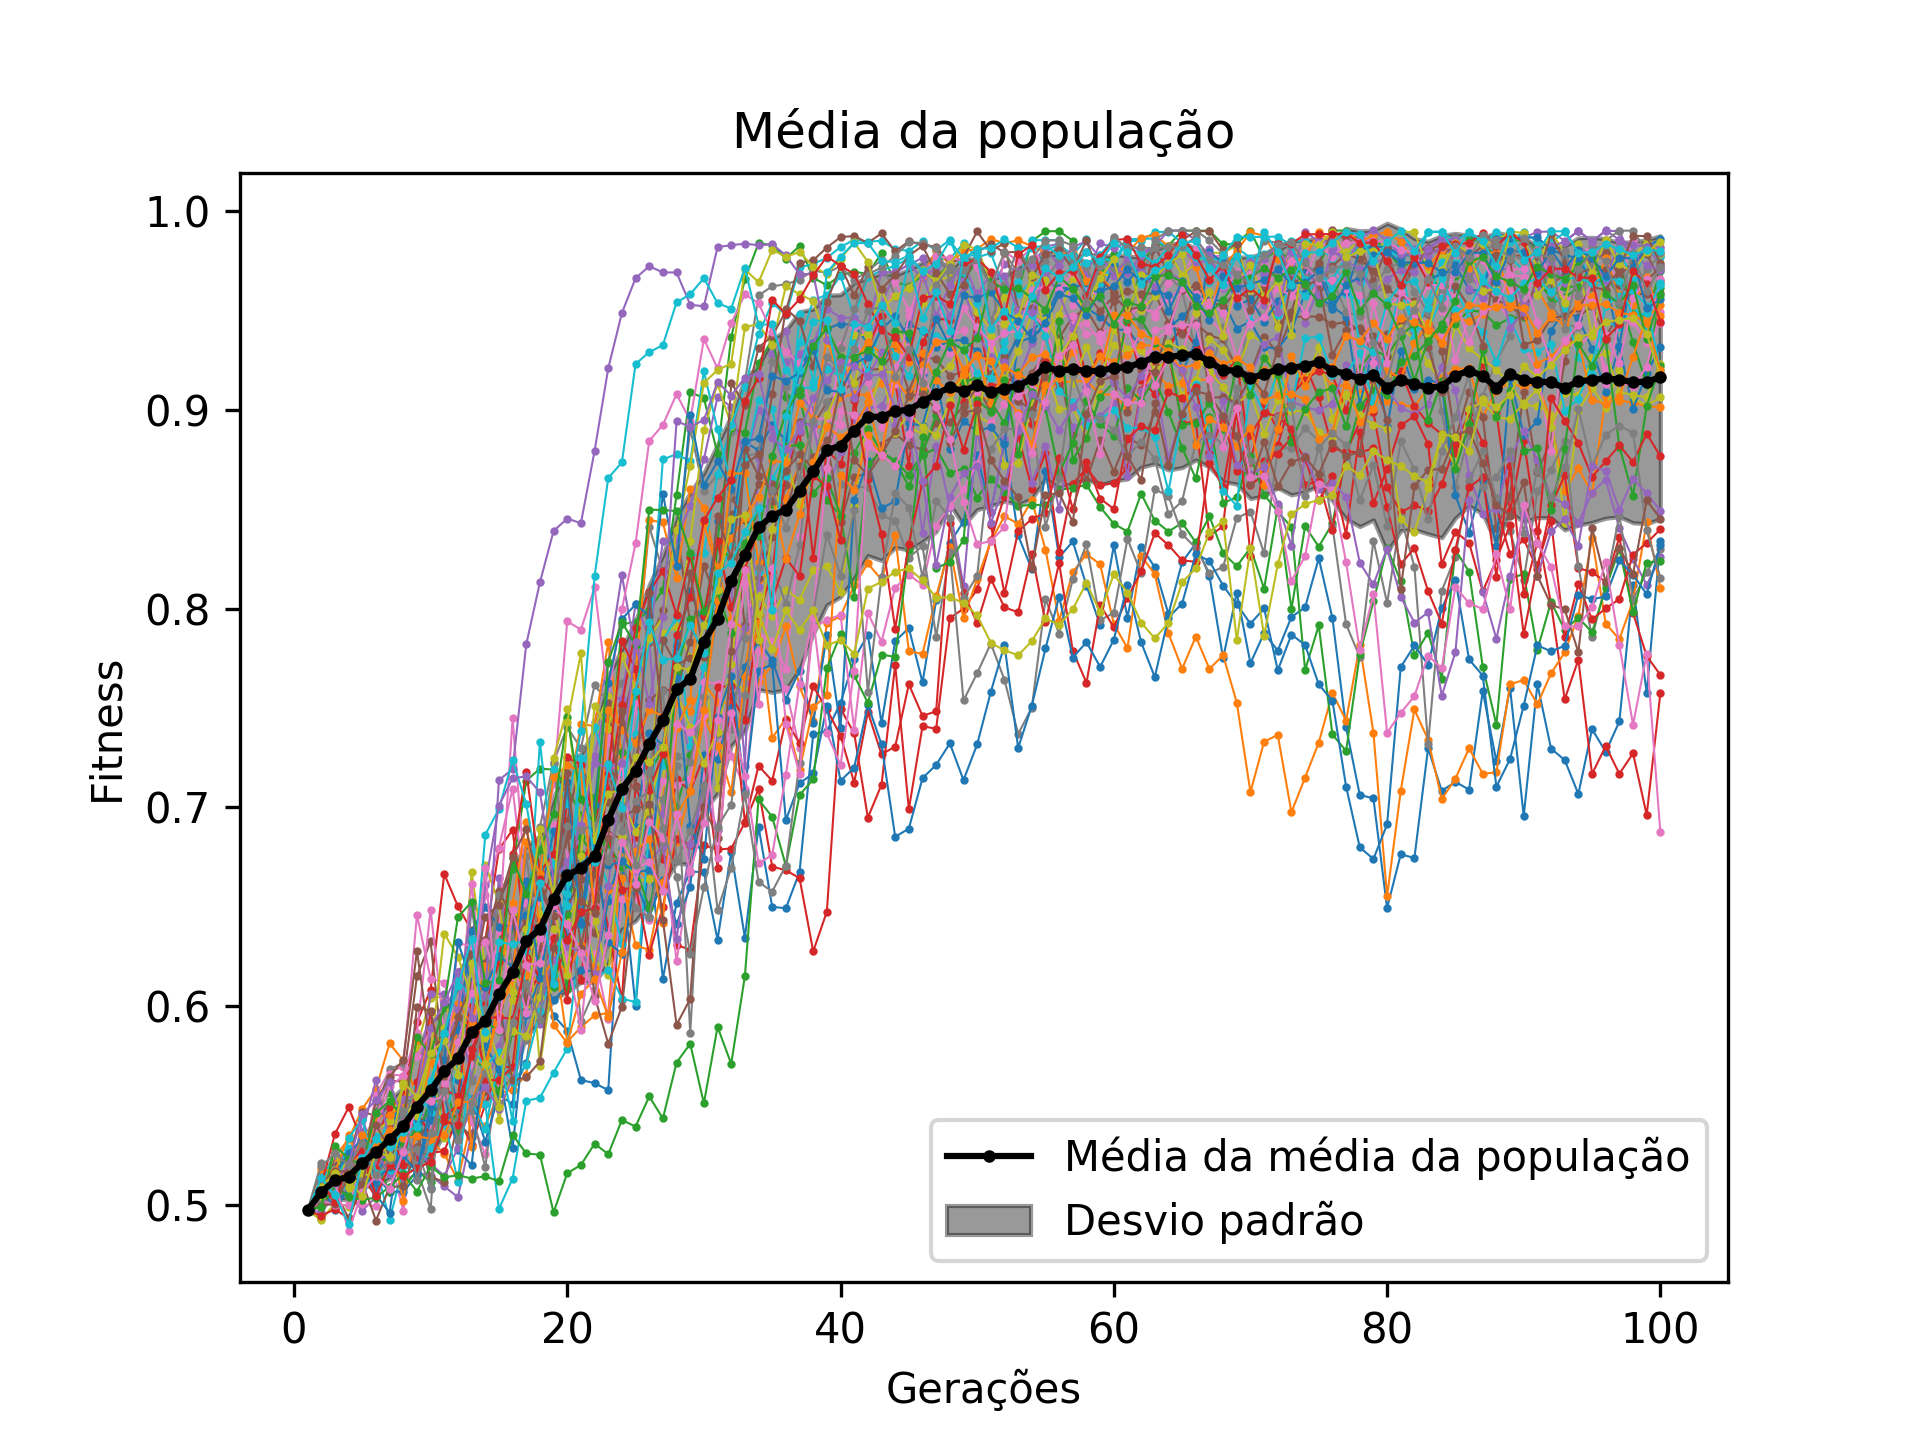
\includegraphics[width=1\textwidth]{sec-03/f6_real_elite_fitness_vs_gen_pop.png}
		\caption{Média da população de todos os experimentos ao longo das gerações.
		Em preto é mostrado o comportamento médio dos 50 experimentos.}
	\end{subfigure}
	\caption{Resultados obtidos utilizando representação real, cruzamento aritmético,
    mutação uniforme e elitismo}
\end{figure}